\begin{figure}[h!]
    \centering
        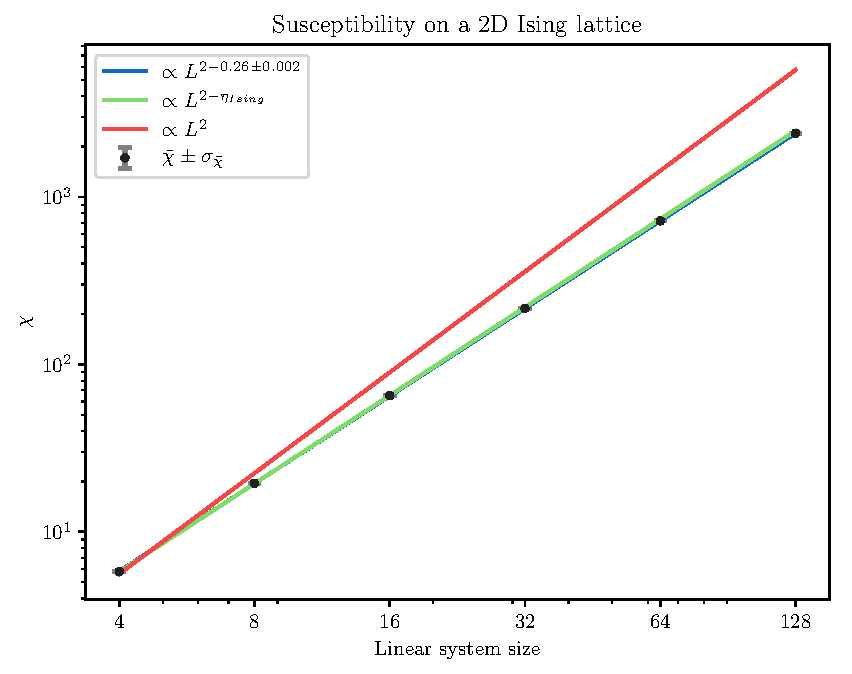
\includegraphics[width=0.8\textwidth]{figures/susceptibility128x128Ising.pdf}
    \caption{Scaling of susceptibility at $T_c$ on an Ising lattice of varying sizes. The measured critical exponent $\eta = 0.26 \pm 0.002$ is compared to the theoretical value $\eta_{Ising} = 0.25$. The red line labeled $\propto L^2$ is there for comparison.}
    \label{fig:results_isingsusc}
\end{figure}

\begin{figure}[h!]
    \centering
        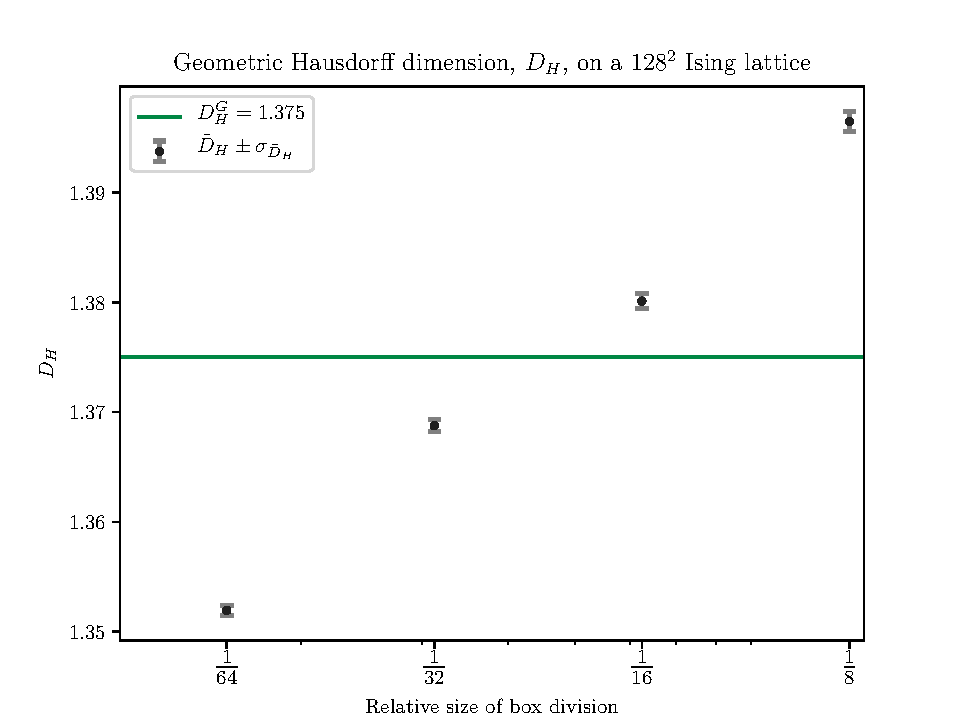
\includegraphics[width=0.8\textwidth]{figures/box_dim_128x128Ising.pdf}
    \caption{Estimation of the Hausdorff dimension of the longest worm loop on a $128^2$ Ising lattice at $T_c$ using the box dimension. The $x$ axis show the size of one box relative to the side length of the lattice. The green line indicates the theoretical dimension of the geometric Ising cluster, $D_H^G = 1.375$.}
    \label{fig:results_boxdimension}
\end{figure}

\begin{figure}[h!]
    \centering
        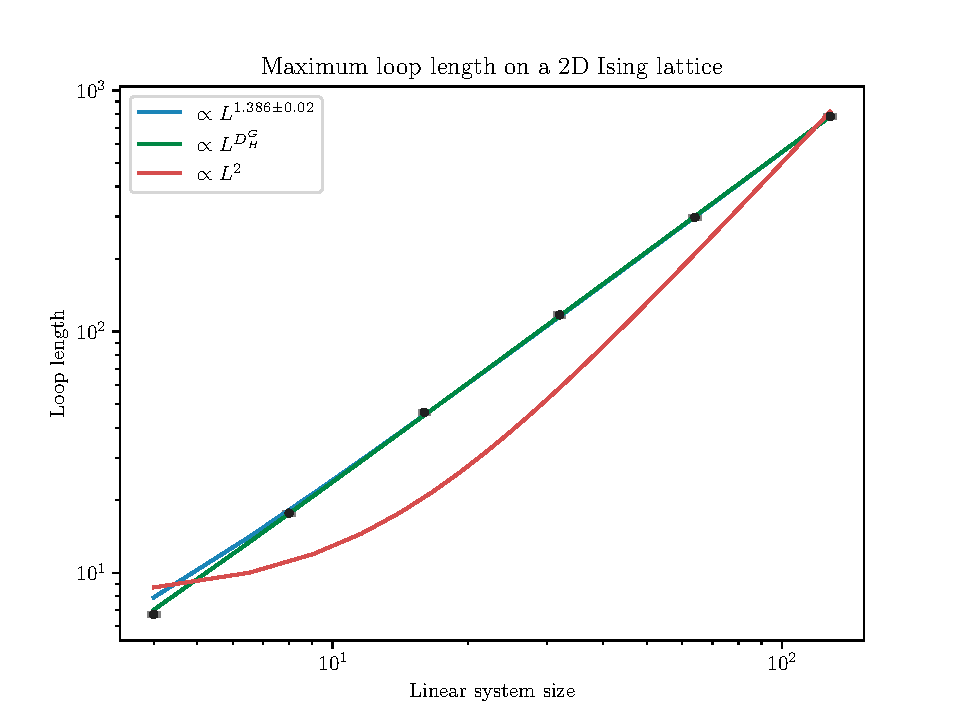
\includegraphics[width=0.8\textwidth]{figures/maximum_loop_length_for_2D_Ising.pdf}
    \caption{Log-log plot of the longest worm loop at $T_c$ on an Ising lattice of varying sizes. The measured scaling factor is $1.386 \pm 0.02$ compared to the theoretical Hausdorff dimension of $1.375$. The red plot labeled $\propto L^2$ is there for comparison.}
    \label{fig:results_maxloopdimension}
\end{figure}


\begin{figure}[h!]
    \centering
        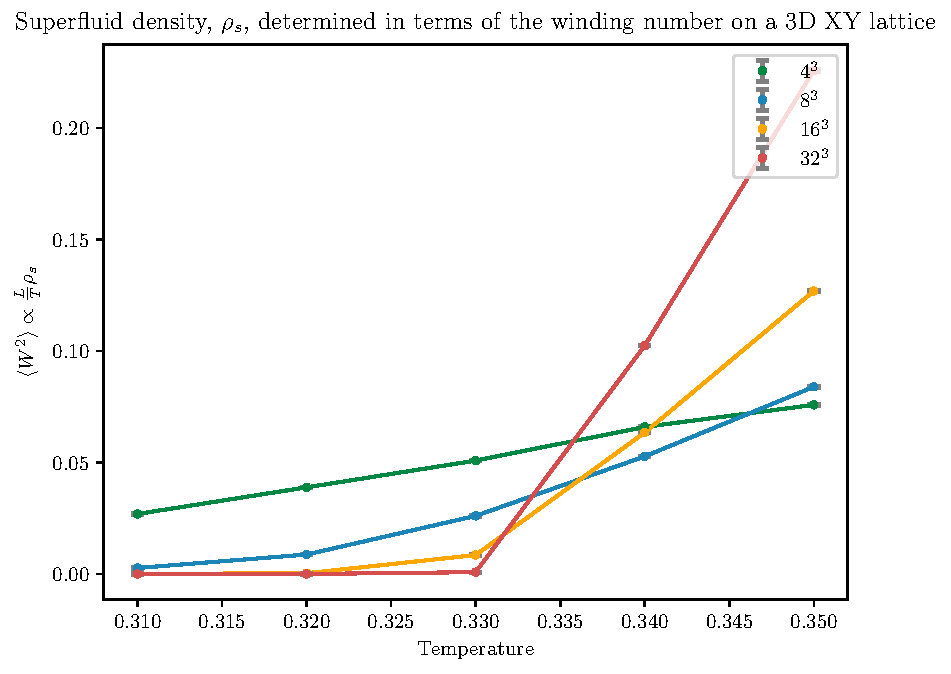
\includegraphics[width=0.8\textwidth]{figures/winding_number_Tc.pdf}
    \caption{Average winding number squared, $\langle W^2 \rangle \propto \rho_s$, plotted on a 3D XY lattice of varying sizes. Due to the Villain approximation the transition is flipped such that $\rho_s \neq 0$ for $T > T_c$, and $T_c$ is translated from $\approx 2.2$ to $\approx 0.333$ indicated by the intersection.}
    \label{fig:results_windingnumberTc}
\end{figure}

